\newpage

%===============================================[Section: Non-Linear Forecasting
\section{METHODS}
%This section will use the Lorenz system to describe the non-linear forecasting technique. The set of differential equations that describes the Lorenz system is introduced and the concept of a phase space is discussed. From there, the nonlinear forecasting technique is illustrated by rebuilding a phase space from only a single variable of the Lorenz system and using the rebuilt phase space to make forecasts. Finally, the forecasting skill is analyzed over a number of parameters that elucidate properties of the original Lorenz system.
%===============================================[Subsection: Lorenz System]
\subsection{THE LORENZ SYSTEM}

The well-known Lorenz equations will be used as an initial illustration of the nonlinear forecasting technique.  The Lorenz equations comprise a coupled dynamical system that represent a simple model of two-dimensional fluid flow when forced by a temperature gradient \cite{lorenz_equations}. Formally, the Lorenz equations are given by
$$ \frac{dx}{dt} = \sigma(y-x), $$
$$\frac{dy}{dt} = x( \rho - z ) - y, $$
$$\frac{dz}{dt} = xy - \beta z,$$
where $x$ is related to the rotational speed of the flow, $y$ is proportional to temperature differences between  rising and sinking flows, $z$ is the deviation of temperature from the mean, $\sigma$ is the fluid viscosity, $\rho$ is the Rayleigh number, and $\beta$ is the ratio of width to height of the fluid. The numerical solutions to these equations with $\rho=28$, $\sigma=10$, and $\beta=\frac{8}{3}$ produce time series  (Figure \ref{individual_lorenz_sols}) with classic hallmarks of deterministic chaos, namely sensitivity to initial conditions and saturated spectrums. Sensitivity to initial conditions is illustrated here by solving the system of equations, having started from slightly different initial conditions, and plotting the difference in system evolution for each dynamical variable (Figure \ref{lorenz_diff}). The difference between the two solutions is initially small, but the solutions exponentially diverge from each other and the initially small variation quickly approaches the bounding size of the system. 

\begin{figure}[htbp]  % FIGURE
   \centering
   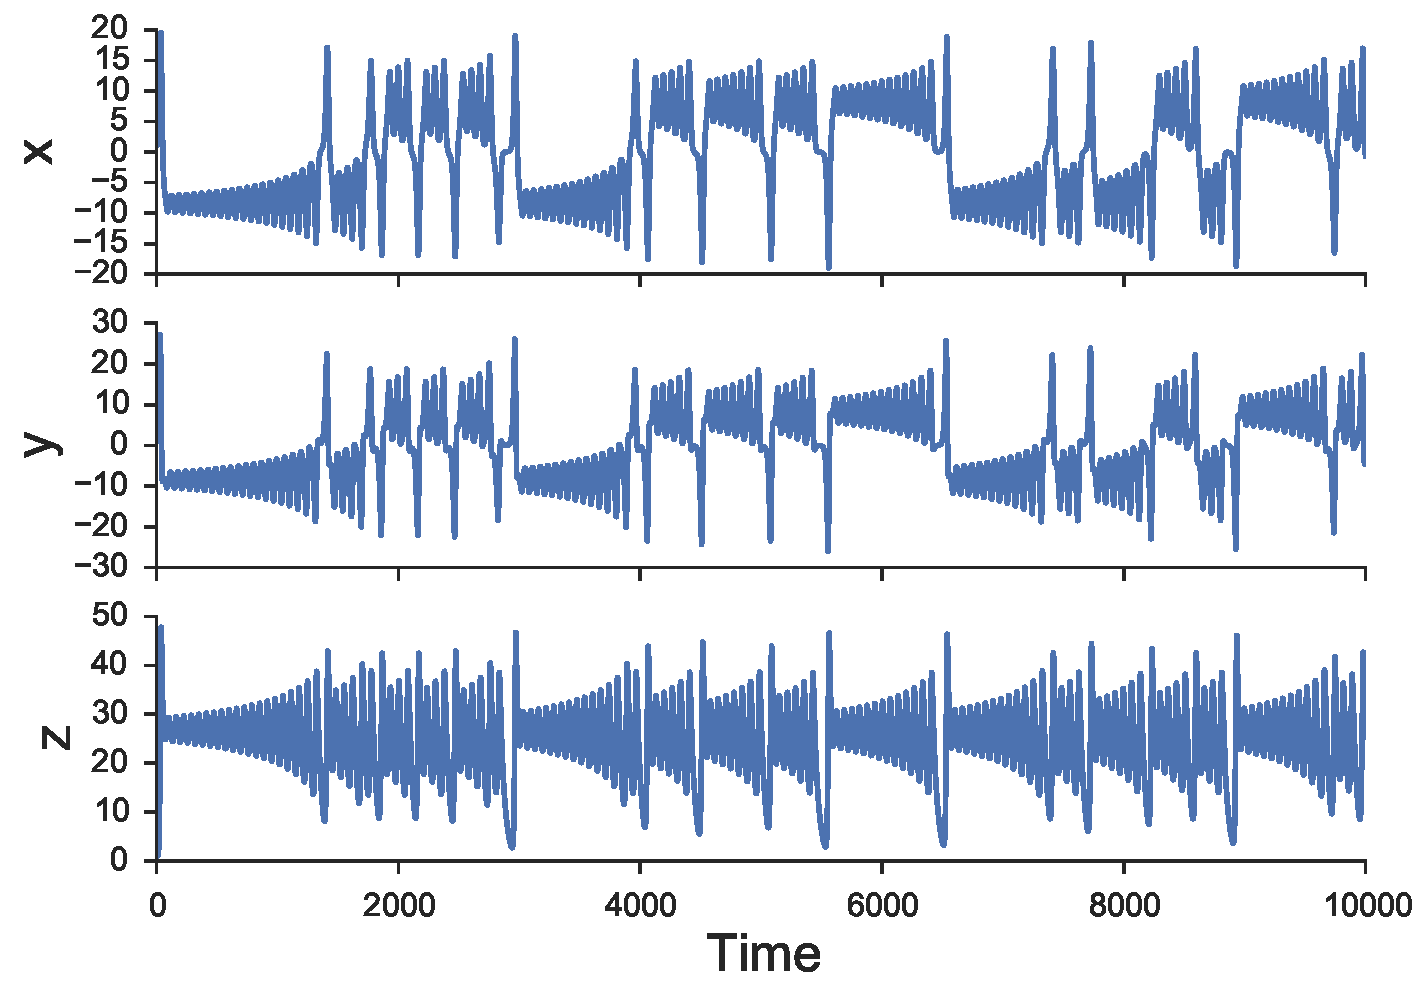
\includegraphics[width=4 in]{lorenz/individual_lorenz_series.pdf} 
   \caption{Lorenz system solved with parameters:$\rho=28$, $\sigma=10$, and $\beta=\frac{8}{3}$. }
   \label{individual_lorenz_sols}
\end{figure}


\begin{figure}[htbp]  %FIGURE
   \centering
   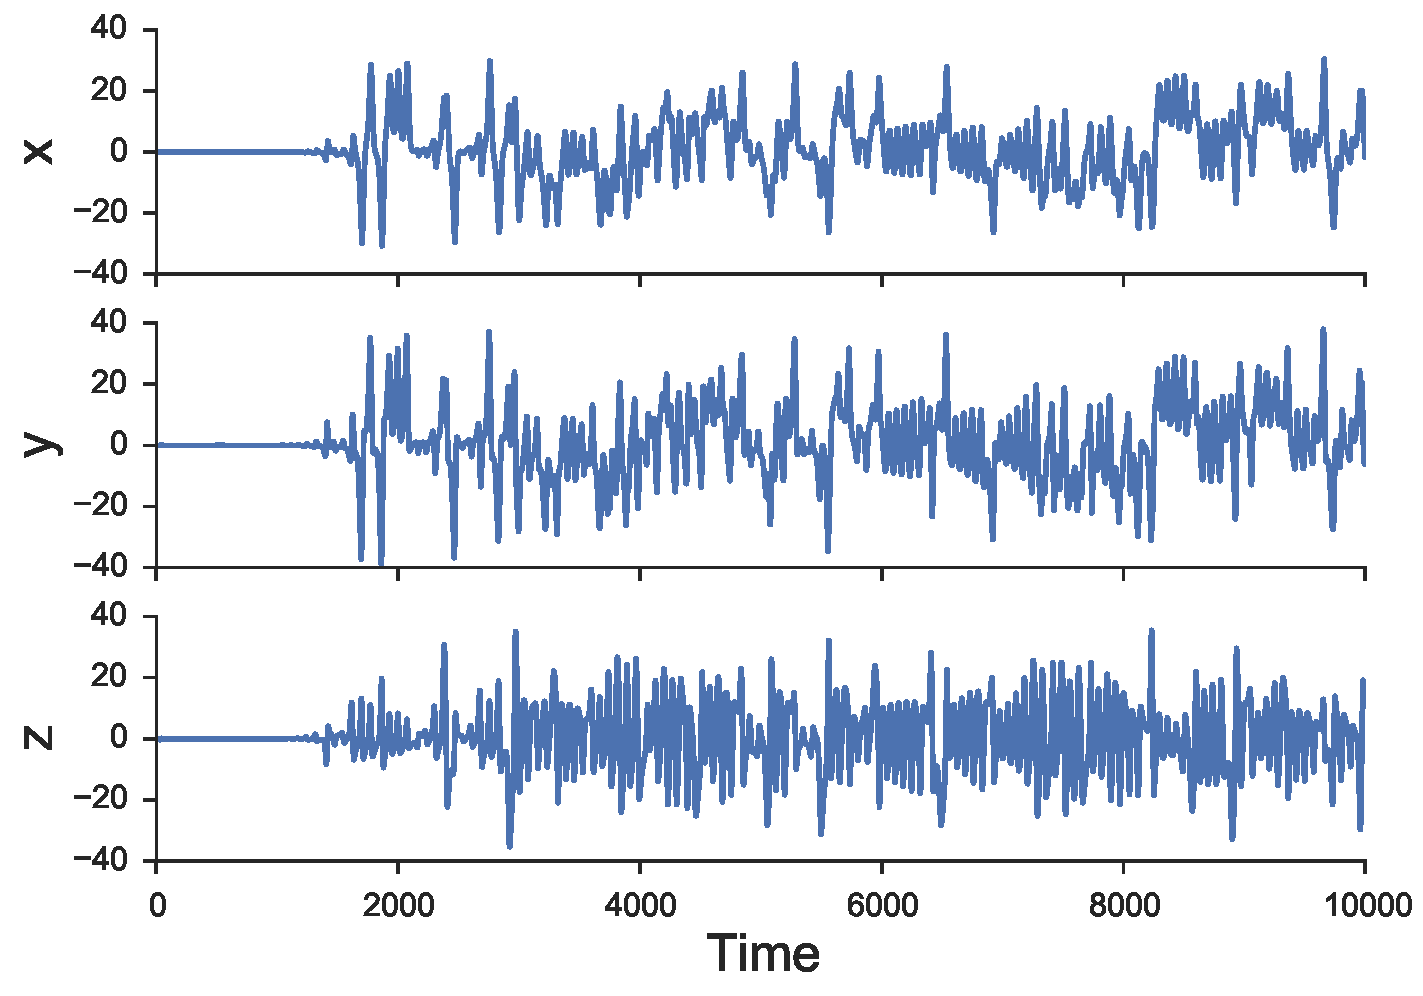
\includegraphics[width=4 in]{lorenz/lorenz_diff.pdf} 
   \caption{Difference between two Lorenz systems solved with parameters:$\rho=28$, $\sigma=10$, and $\beta=\frac{8}{3}$, but started with initial conditions [$X_0 = 1.01$,$Y_0= 1.01$,$Z_0= 1.01$] and [$X_0 = 1.00$, $Y_0= 1.00$, $Z_0= 1.00$]. }
   \label{lorenz_diff}
\end{figure}

A phase space is a space that displays all possible configurations of a system \cite{nonlinear_book}, where the axes of the space represent the variables describing the system. Plotting $X$ vs. $Y$ vs. $Z$ for the Lorenz system shows a single trajectory in the phase space started from the initial condition $[X_0,Y_0,Z_0]$ (Figure \ref{lorenz_butterfly}). Importantly, although trajectories started from different initial conditions diverge, all trajectories for this system remain confined to a subset of the phase space, termed the attractor.  Additionally, trajectories in the phase space can never intersect. Intersection of trajectories would indicate that the system is not deterministic and that a given point in the phase space could evolve in two separate ways. 

\begin{figure}[htbp]  % FIGURE
   \centering
   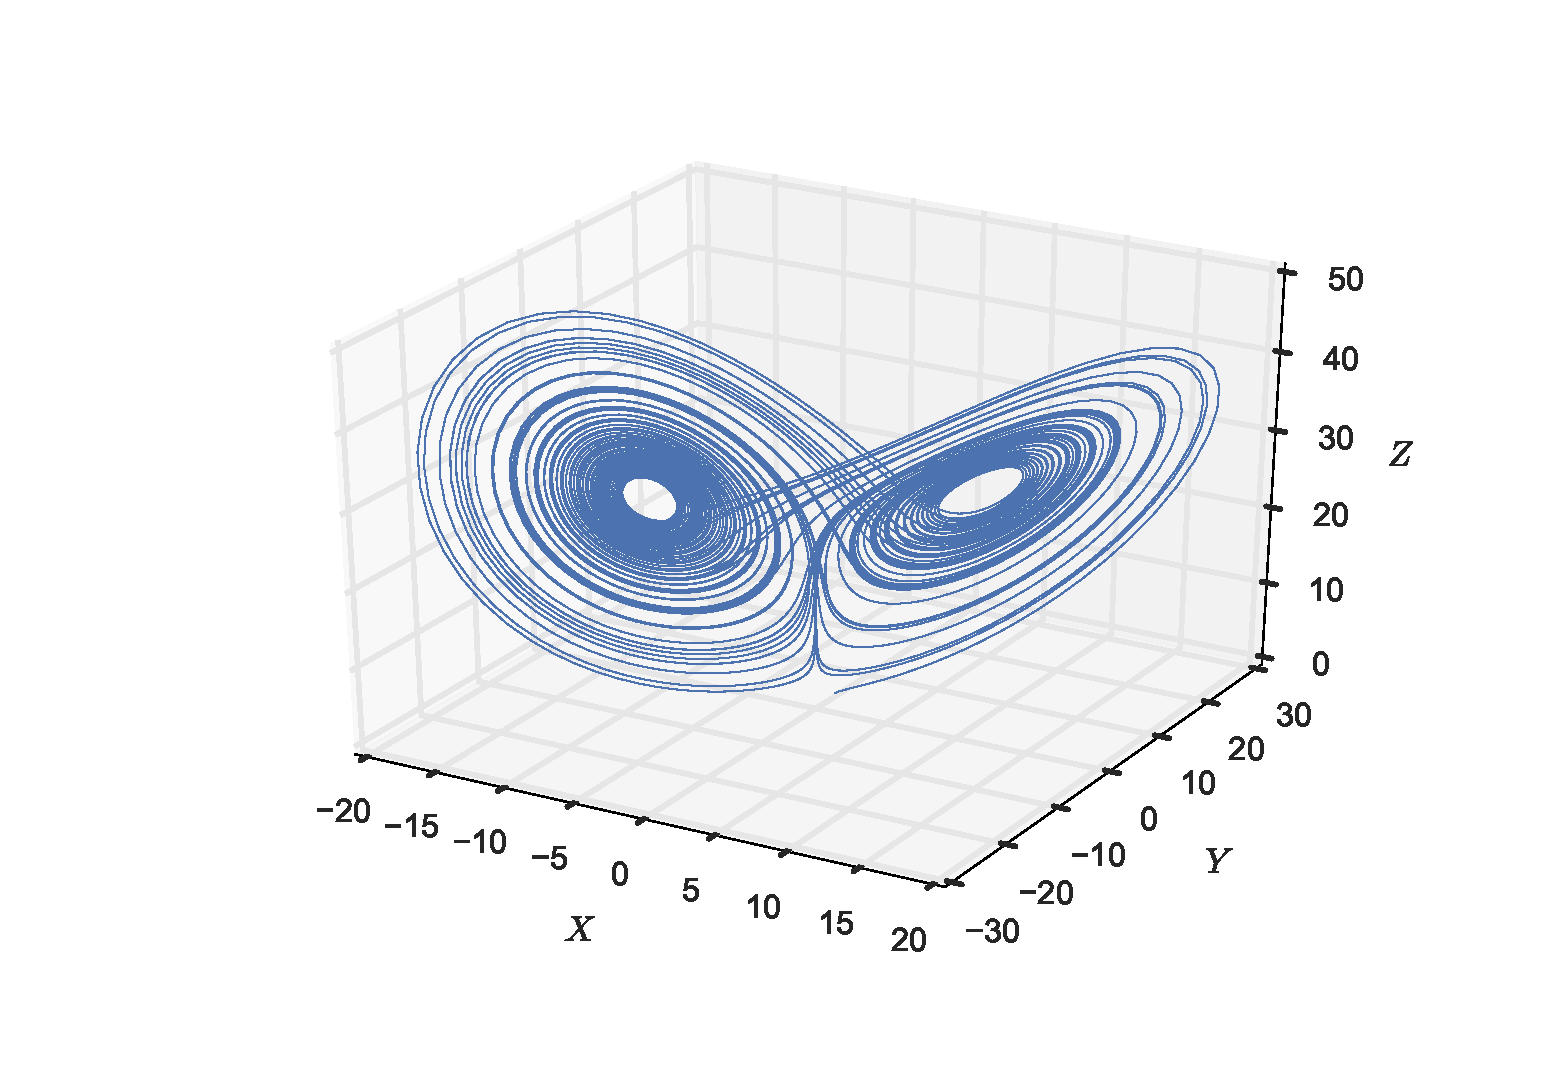
\includegraphics[width=4 in]{lorenz/lorenz_butterfly.pdf} 
   \caption{A single trajectory in the Lorenz phase space solved with parameters:$\rho=28$, $\sigma=10$, and $\beta=\frac{8}{3}$ and started from [$X_0 = 1.00$, $Y_0= 1.00$, $Z_0= 1.00$]. }
   \label{lorenz_butterfly}
\end{figure}


%=========================================================[Subsection: Embedding]
\subsection{RECONSTRUCTED STATE SPACE}
In most natural systems, the underlying dynamical equations that govern a system are unknown.  Often, insight is derived empirically by taking measurements of a single variable. As a proxy for this scenario, imagine having taken measurements of the Lorenz system by only capturing the variable $X$. Florence Taken has shown \cite{takens_theorem} that time lagged values of a single dynamical variable within a multi-dimensional system can be used to reconstruct the basic features of the attractor, a technique termed state space reconstruction. Specifically, although the reconstructed version of the attractor is not identical in appearance, it maintains the dynamically important features of the original attractor such as topology, sensitivity to initial conditions (as measured by the Lyaponov exponent), and attractor dimension. Thus, the reconstructed attractor illuminates the dynamics, or flows within the phase space, through measurements of a single variable. The reconstruction is done by forming vectors, $\vec V_t$, in $m$ dimensional space. These vectors provide a means of embedding  the one dimensional time series into a multi-dimensional space.  Let the embedding vectors be given by 

$$\vec V_t (X) = (X_t, X_{ t - \tau },\dots X_{ t -(m-1) \tau} ).$$

Here $\tau$ represents a fixed lag in time and can be found by calculating the first minimum of the mutual information \cite{mutual_info}.  The embedding dimension can be found by using the false near neighbor test \cite{chaotic_analysis}, however when using this technique on natural time series, the dimension used is more commonly the one which results in the highest forecast skill \cite{embedding_dimension}. For the Lorenz system, the false near neighbor test yields an embedding dimension of three and embedding the $X$  time series in a three dimensional space provides the highest forecast skill.  The reconstructed state space is shown in Figure \ref{embedded_lorenz_x}. 

\begin{figure}[htbp]  %FIGURE
   \centering
   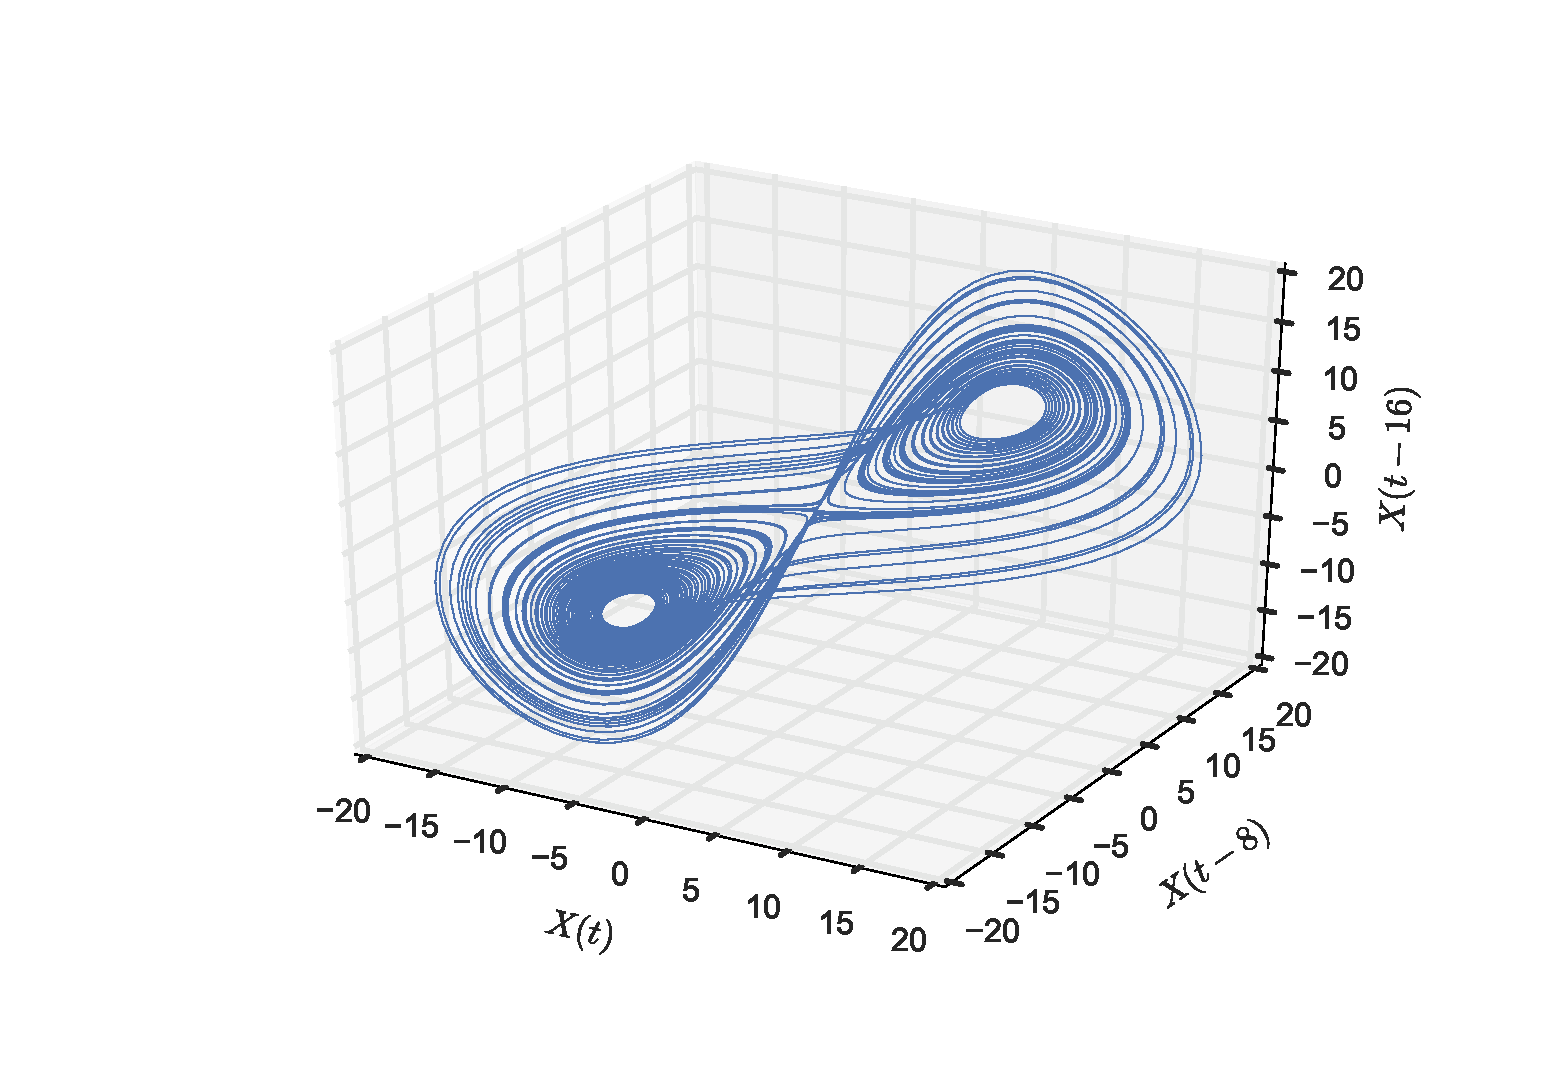
\includegraphics[width=4 in]{lorenz/embedded_lorenz_x.pdf} 
   \caption{Reconstructed state space using $X$ values from the Lorenz system. }
   \label{embedded_lorenz_x}
\end{figure}

The attractor in the reconstructed space qualitatively and quantitatively preserves the same shape as the original Lorenz attractor. Trajectories are smooth and do not cross in the reconstructed space preserving the deterministic nature of the system.

%===================================================[subsection: near neighbor estimates]
\subsection{FORECASTING}

In order to forecast $X_{t+n}$, where n is the forecast distance, the reconstructed state space is used. Given a point  $\vec V_t(X)$, in the embedded space, the $K$ nearest points (near neighbors) are calculated using the euclidean distance. The trajectories of the $K$ nearest neighbors in the embedded space are then averaged and compared to the actual evolution of the point in question.  For the purpose of distinguishing system dynamics, forecasts are made over a range of near neighbors and a range of forecast distances \cite{original_rubin}. In order to quantify the accuracy of the forecasts, the coefficient of determination, $R^2$, is calculated as:

$$ R^2 = 1 - \frac{\sum (y_i - f_i)^2} {\sum (y_i - \bar y)^2},$$
where $y_i$ is the true value, $f_i$ is the forecast value, and $\bar y$ is the mean of the true values. The results of this forecasting technique when applied to the Lorenz system are shown in Figure \ref{lorenz_contour}.


\begin{figure}[htbp]  %FIGURE
   \centering
   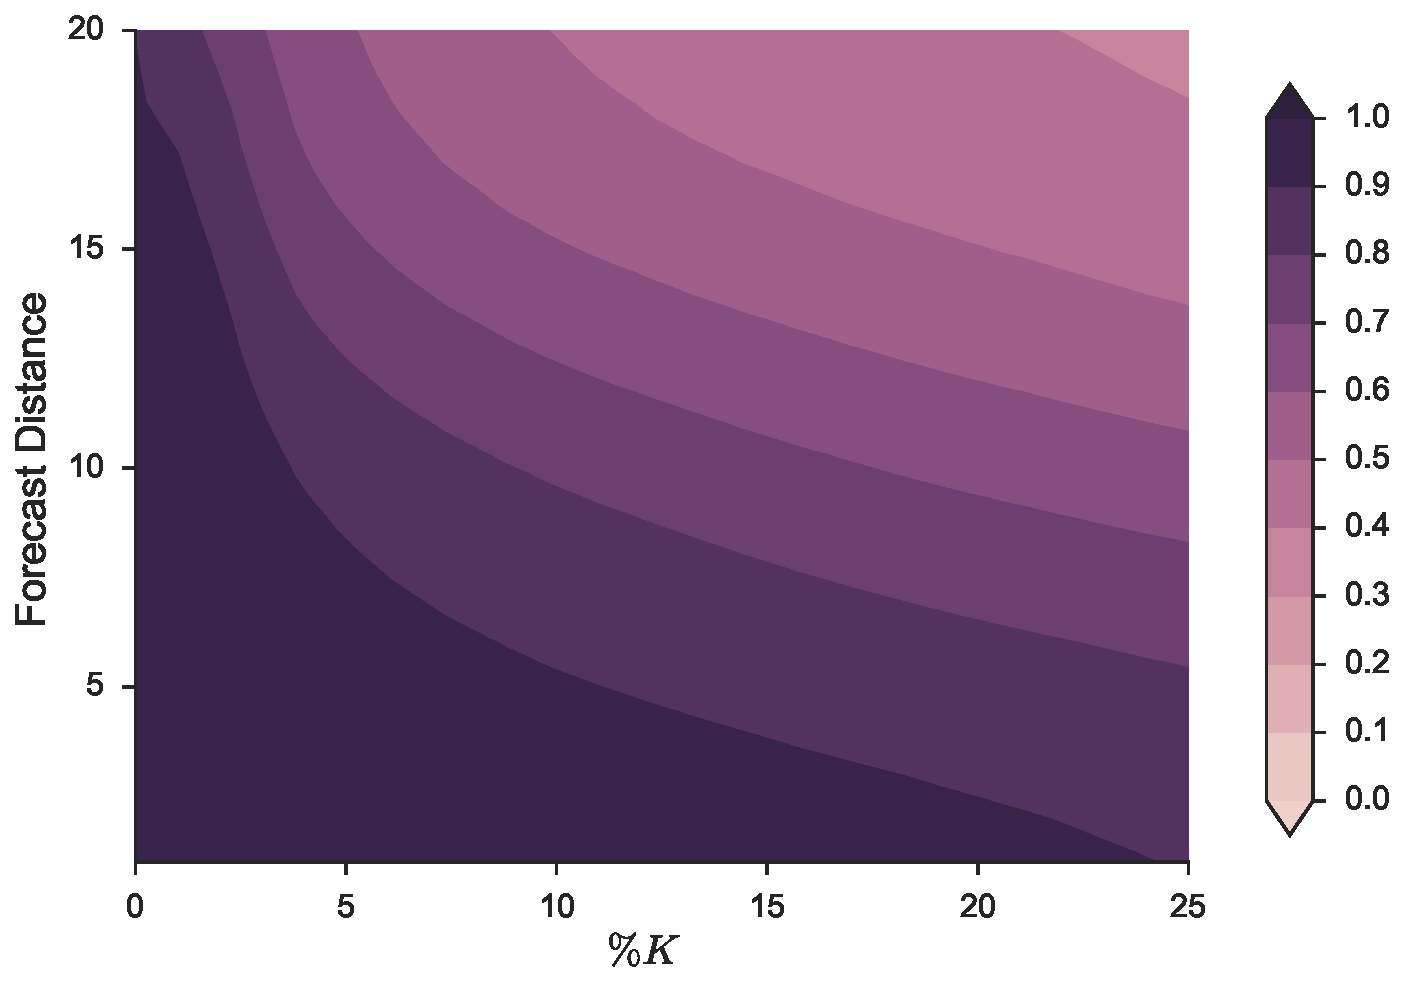
\includegraphics[width=4 in]{lorenz/forecasted_lorenz_x.pdf} 
   \caption{The coefficient of determination ($R^2$) plotted against near neighbors ($K$) and forecast distance.}
   \label{lorenz_contour}
\end{figure}

Figure \ref{lorenz_contour} captures the Lorenz system's sensitivity to initial conditions as evident by the decreasing $R^2$ value with increasing forecast distance.  Deterministic nonlinearity is evident by the decrease of forecast skill when increasing the number of near neighbors used in the forecast.  This trend reflects the importance of localized flow dynamics within the phase space as trajectories that are farther away from a test forecasting point are less accurate representations of future behavior.


%============================================================[Deterministic Metric]
\subsection{EVALUATING DETERMINISM}

In order to evaluate the amount of stochasticity in a system, increasing amplitudes of uncorrelated noise are added to the embedded Lorenz $x$ values as,

$$x_n = x + \alpha\eta,$$
where $x_n$ is the Lorenz $x$ values with added noise, $\alpha$ is the amplitude of the noise, and $\eta$ is uncorrelated noise having values between zero and one. The noise complicates trajectories in the state space as the original smooth trajectories become jagged and overlapping. An example of a reconstructed state for $x_n$ is shown in Figure \ref{rebuilt_noise}. The non-linear forecasting technique is applied and the results are shown in Figure \ref{lorenz_metric_contour}. 

\begin{figure}[htbp]  %FIGURE
   \centering
   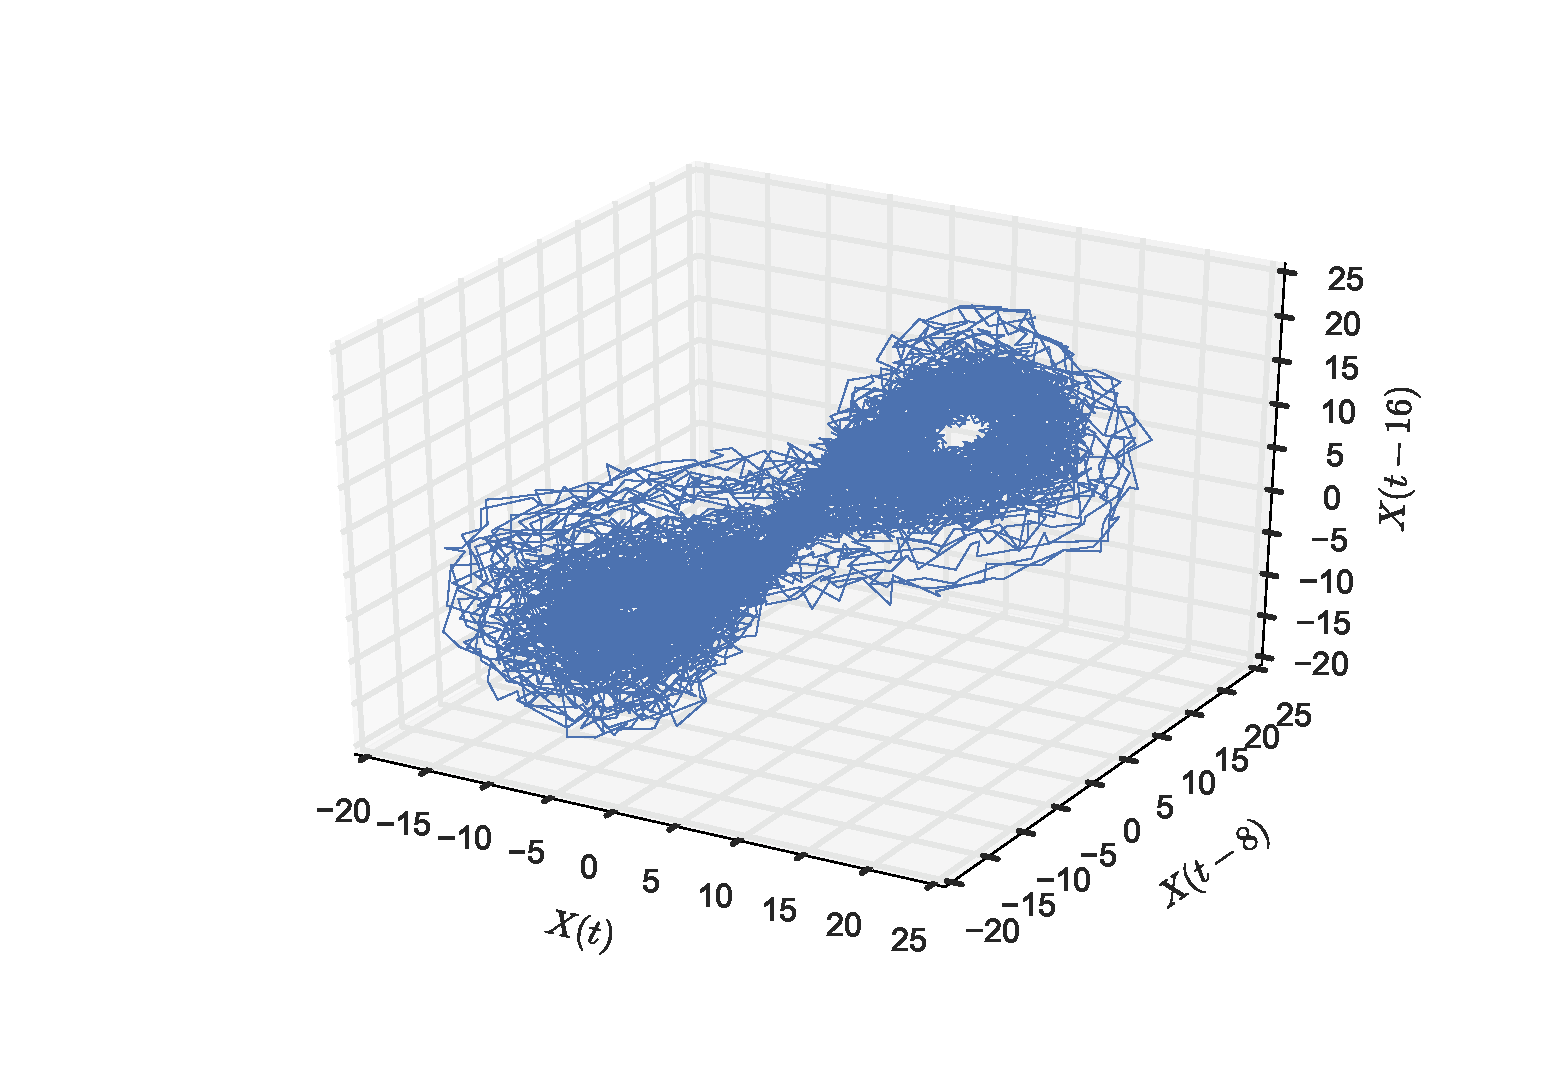
\includegraphics[width=4 in]{lorenz/embedded_lorenz_x_noise.pdf} 
   \caption{The embedded $x$ time series from the Lorenz system with uncorrelated noise added to the time series. }
   \label{rebuilt_noise}
\end{figure}

\begin{figure}[htbp]  %FIGURE
   \centering
   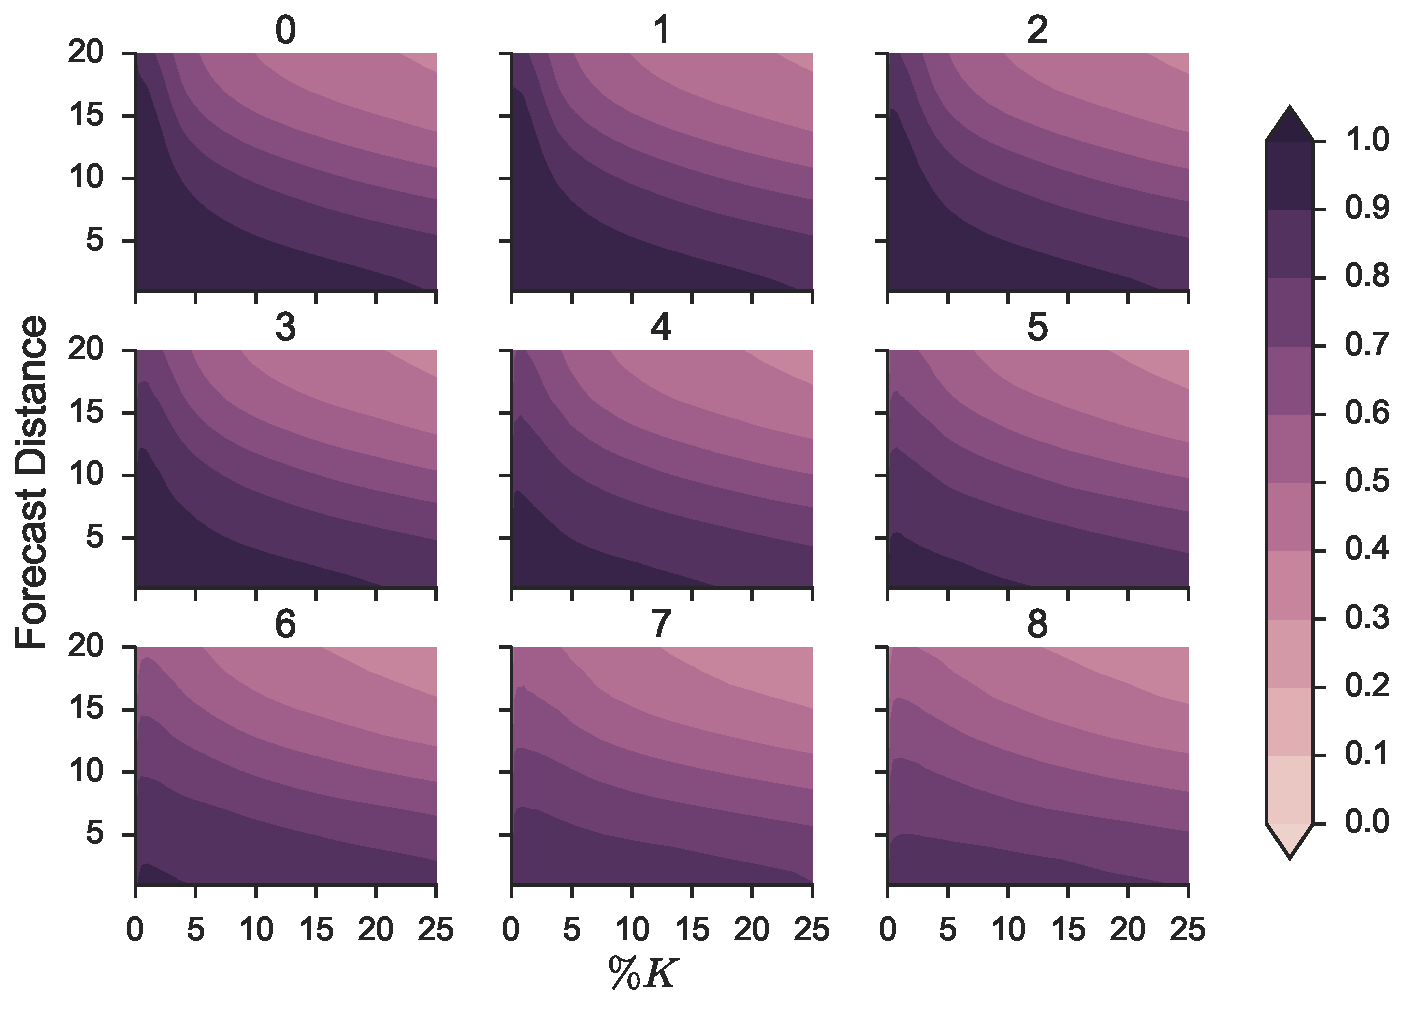
\includegraphics[width=4 in]{lorenz/lorenz_contours.pdf} 
   \caption{The coefficient of determination ($R^2$) plotted against near neighbors ($K$) and forecast distance. Title corresponds to the amplitude of the noise, $\alpha$. }
   \label{lorenz_metric_contour}
\end{figure}



A simple metric is created that attempts to calculate the relative contributions of determinism and randomness in a system. In order to apply the metric, two assumptions must be made. First, the systems being compared must have the same underlying dynamics. For example, comparing the amount of determinism in a coastal formation to the amount of determinism in a biological pattern would not be valid. Conversely, comparing the amount of determinism across different biological patterns within the same system or comparing the amount of determinism across different coastal formations could provide insight. The second assumption is that the phase space is well populated within the system attractor.

The goal of the metric is to collapse the contours in Figure \ref{lorenz_metric_contour} into a single value. To capture the high forecast skill at low $K$ for deterministic systems, the metric is represented as:

$$ D = \sum^n_{d=1} max(R^2_{d,\%K<12.5}) - min(R^2_{d,\%K\geq12.5}), $$
where $D$ is the deterministic metric, $d$ is the forecast distance, $n$ is equal to one-half of the mutual information of the system, $\%K$ is the percent of near neighbors, and $R^2$ is the coefficient of determination. For each forecast distance, the metric calculates the maximum $R^2$ value at low numbers of near neighbors and subtracts the minimum $R^2$ value at high near neighbors. It then sums up the differences out to a forecast distance that is one-half of the mutual information of the system. The metric is run on the nine contour plots in Figure \ref{lorenz_metric_contour} and the results are shown in Figure \ref{lorenz_metric_bar}. 

\begin{figure}[htbp]  %FIGURE
   \centering
   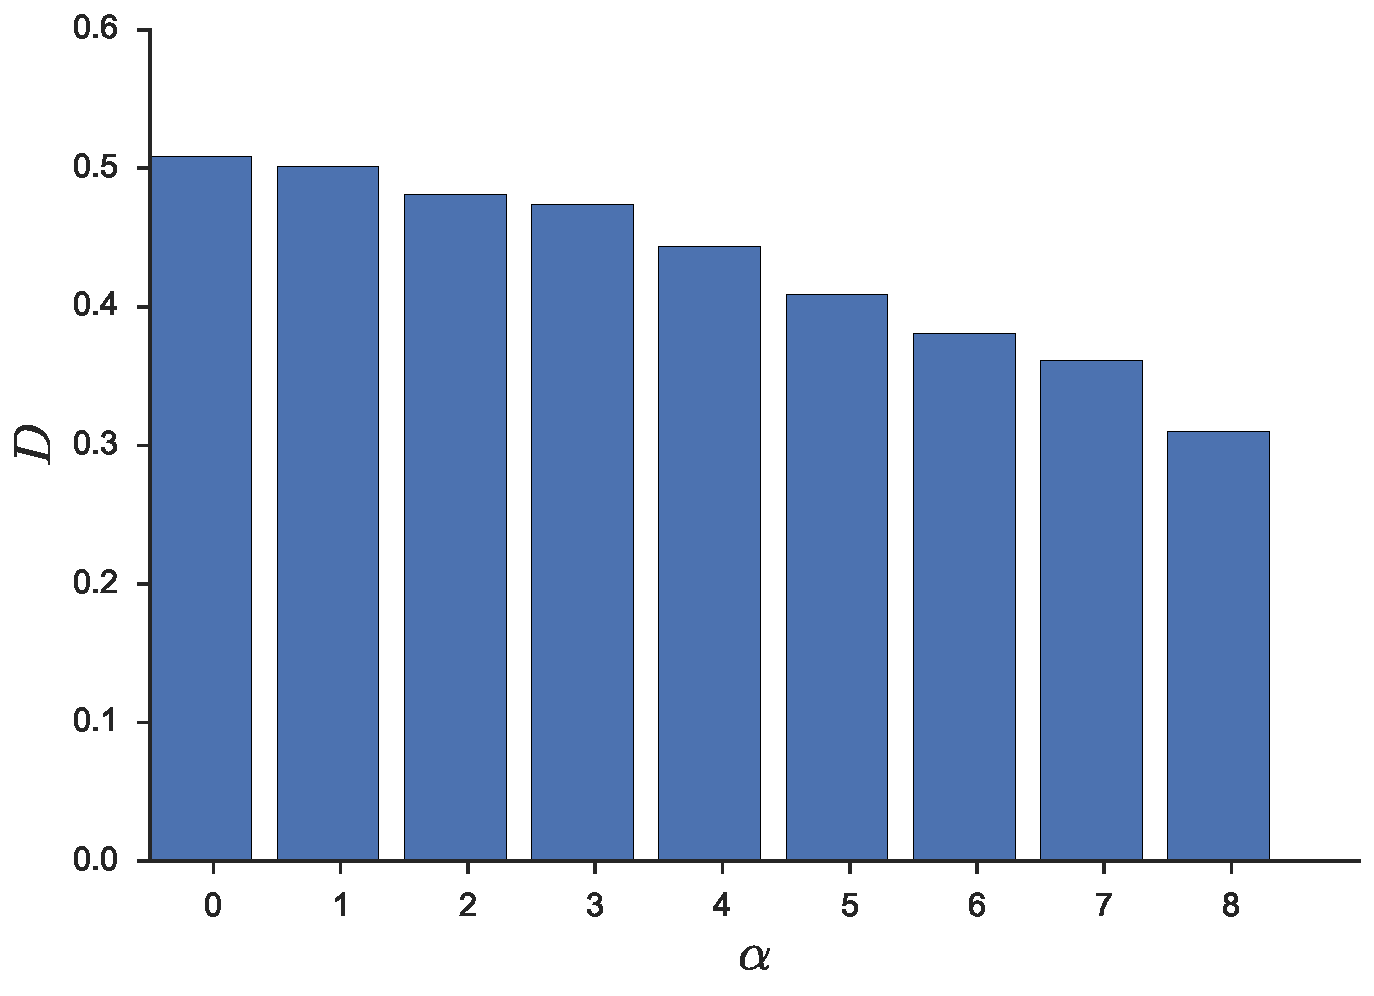
\includegraphics[width=4 in]{lorenz/lorenz_bar_plot.pdf} 
   \caption{The deterministic metric calculated from the Lorenz system. The $x$-axis corresponds to the amplitude of the noise, $\alpha$.}
   \label{lorenz_metric_bar}
\end{figure}

The larger the relative role of determinism versus noise,the larger the value of $D$. The metric captures the fact that stochastic systems benefit from averaging higher amounts of near neighbor trajectories in forecasting system behavior while systems with stronger deterministic dynamics benefit from averaging trajectories near in the reconstructed state space. 

%=================================================[subsection: conclusion]
%\subsection{CONCLUSION}
%
%In this section, the non-linear forecasting technique was described and applied to the Lorenz series and the system was forecasted over a range of near neighbors and prediction distances for the $X$ variable. Patterns emerged in Figure \ref{lorenz_contour} that illustrate the system's sensitivity to initial conditions. The lower $R^2$ values at larger forecast distances were not due to any noise in the system. In the next sections, other systems will be explored and the patterning in their contour plots will be analyzed and more definite statements about determinism will be be made.









%